%% -----------------------------------
%%
%%
%% Copyright (C)
%%     2022     by latexstudio.net
%%
%%
\documentclass[12pt]{article}
%% 导言区
%%=============setting,设置自己的队号和选题============
\gdef\MCMcontrol{2019057552}%队号
\newcommand{\problem}{C}%选题

\newcommand{\control}{\MCMcontrol}
\newcommand{\team}{Team \#\ \MCMcontrol}
\newcommand{\headset}{{\the\year}\\MCM/ICM\\Summary Sheet}

%==========定义摘要,摘要的标题可自定义===================
\renewenvironment{abstract}[1]{%
	\small
	\begin{center}%
		{\large\bfseries #1\vspace{-.5em}}%
\end{center}}
{}
\newcommand\keywords[1]{%
	\begingroup
	\par
	\noindent\textbf{Keywords:} #1\par
	\endgroup
}

% 目录居中的重定义
\makeatletter
\renewcommand\tableofcontents{%
	\centerline{\normalfont\Large\bfseries\contentsname%
		\@mkboth{%
			\MakeUppercase\contentsname}{\MakeUppercase\contentsname}}%
	\vskip 3ex%
	\@starttoc{toc}%
	\thispagestyle{fancy}
	\clearpage}
\makeatother

\usepackage[toc, page, title, titletoc, header]{appendix}
\usepackage{graphicx}
\graphicspath{{figures/}{img/}}

\usepackage{amsmath,amssymb,amsfonts,amsthm}
\newtheorem{Theorem}{Theorem}[section]
\newtheorem{Lemma}[Theorem]{Lemma}
\newtheorem{Corollary}[Theorem]{Corollary}
\newtheorem{Proposition}[Theorem]{Proposition}
\newtheorem{Definition}[Theorem]{Definition}
\newtheorem{Example}[Theorem]{Example}


%==========设置代码格式===================
\usepackage{xcolor}
\usepackage{listings}
\definecolor{grey}{rgb}{0.8,0.8,0.8}
\definecolor{darkgreen}{rgb}{0,0.3,0}
\definecolor{darkblue}{rgb}{0,0,0.3}
\def\lstbasicfont{\fontfamily{pcr}\selectfont\footnotesize}
\lstset{%
	% numbers=left,
	% numberstyle=\small,%
	showstringspaces=false,
	showspaces=false,%
	tabsize=4,%
	frame=lines,%
	basicstyle={\footnotesize\lstbasicfont},%
	keywordstyle=\color{darkblue}\bfseries,%
	identifierstyle=,%
	commentstyle=\color{darkgreen},%\itshape,%
	stringstyle=\color{black}%
}
\lstloadlanguages{C,C++,Java,Matlab,Mathematica}

\usepackage{geometry}
\geometry{a4paper, margin = 1.2in}

%==========设置页眉格式===================
\usepackage{fancyhdr,lastpage}
\pagestyle{fancy}
\fancyhf{}
\lhead{\small\sffamily \team}
\rhead{\small\sffamily Page \thepage\ of \pageref{LastPage}}
\setlength\parskip{.5\baselineskip}

\usepackage{hyperref}
\usepackage{mathptmx}% newtxtext
\usepackage{lipsum}
\title{The \LaTeX{} Template for MCM Version 1}
\author{\small \href{http://www.latexstudio.net/}
	{
\includegraphics[width=7cm]{mcmthesis-logo}}}
\date{\today}
\usepackage{pdfpages}
\usepackage{tikz}
\begin{document}
	%% 摘要环境
	% \subfile{./segments/abstract_}
	\newpage
	\tableofcontents
	% use for demo
    % list environment like paragraph
    \begin{enumerate}[label=, leftmargin=0pt, itemindent=\parindent]
        \item \lipsum[1]
        \item \lipsum[2]
    \end{enumerate}
	% no float note table
    \begin{minipage}{\linewidth}
    \begin{threeparttable}[b]
    	\begin{tblr}{
	        width=\linewidth,
            colspec={X[-1, c]XX[6, c]},
            hline{1, Z} = {2pt, solid}, 
            hline{2} = {solid}
        }
        Symblo && Description\\
    \end{tblr}
        \begin{tablenotes}[flushleft]
        	\item Note: The above table does not list all symbols, the meaning of the symbol is subject to the use of the symbol.
        \end{tablenotes}
    \end{threeparttable}
    \end{minipage}
    % no folat table
    \begin{minipage}{1.0\linewidth}
    \captionof{table}{Examples of untrustworthy comments}
    \label{tab:4.1.1}
    \begin{tblr}{
          width=\linewidth,
          colspec={*{6}{X[c]}},
          hline{1, Z} = {2pt, solid},
          hline{2} = {solid}
        }
        marketplace & customer\_id & … & vine & verified\_purchase & …  & review\_date \\
        US & 39431051 & … & N & N & … & 8/31/2015\\
    \end{tblr}
    \end{minipage}
    % subfigure useage
     \begin{figure}[!ht]
    \centering
    \subfigure[pacifier\_star\_ratio]{
       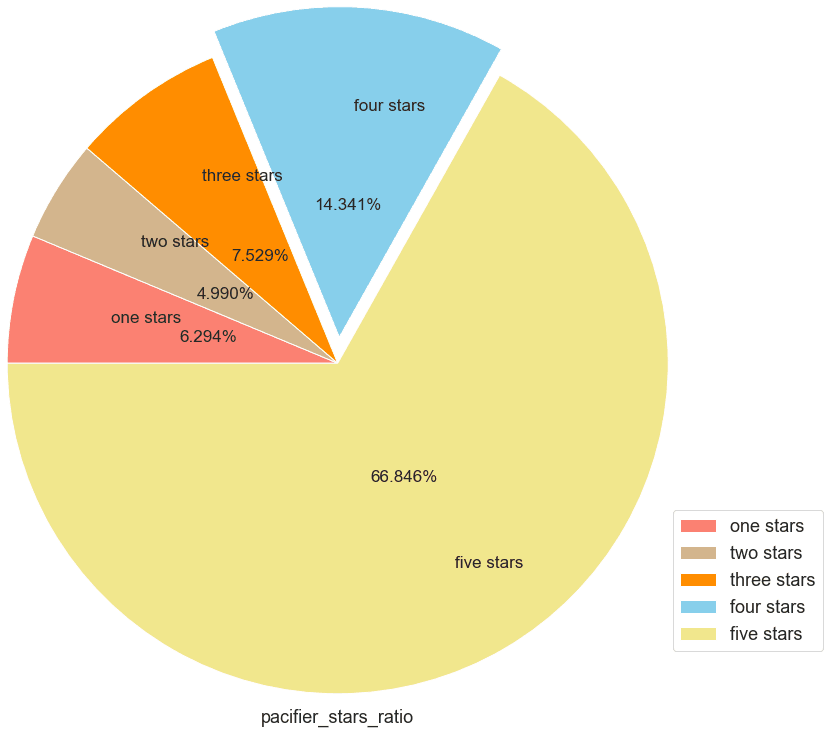
\includegraphics[scale=0.12]{4.2.1}
    }
    \qquad
	\subfigure[hair\_dryer\_star\_ratio]{
      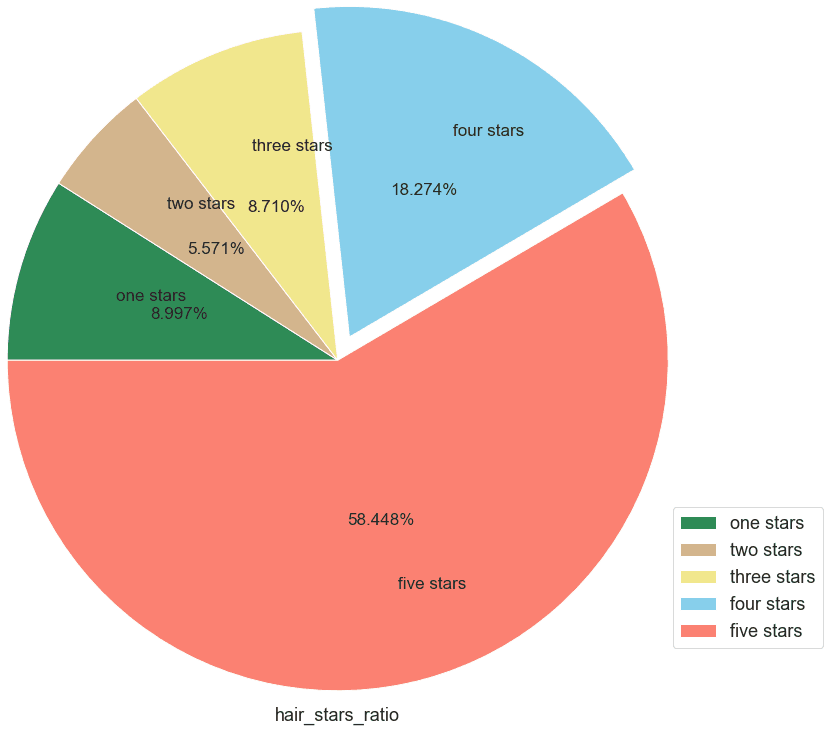
\includegraphics[scale=0.12]{4.2.2}
    }
    \qquad
    \subfigure[microwave\_star\_ratio]{
      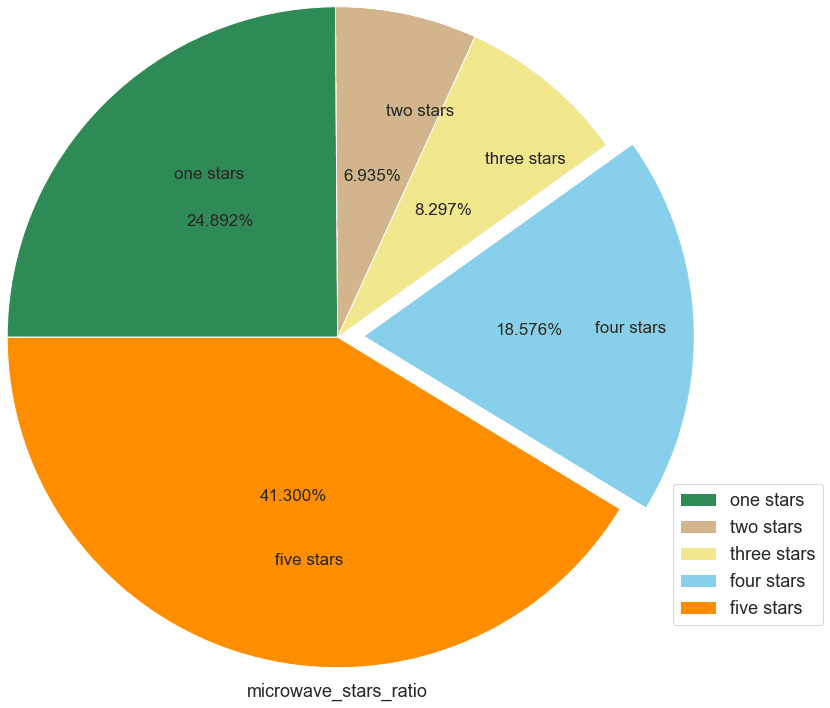
\includegraphics[scale=0.12]{4.2.3}
    }
    \captionof{figure}{The proportion of five stars in the star\_rating of each product}
    \label{fig:4.2.1}
    \end{figure}
    % no float figure
    \begin{minipage}{1.0\linewidth}
    \centering
    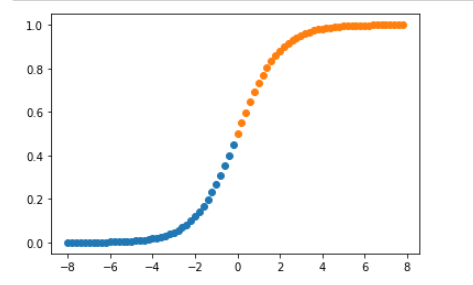
\includegraphics[scale=0.5]{4.2.4}
    \captionof{figure}{Image of sigmoid function}
    \label{fig:4.2.4}
    \end{minipage}
    \includepdf{../../Downloads/need.pdf}
	%==========设置正文格式===================
	
	\subfile{./segments/introduction_}
	
	% 分析
	\subfile{./segments/analysis_}
	
	% 计算
	\subfile{./segments/calculate_}
	
	% 模型结果
	\subfile{./segments/model_result}
	
	% %
	\subfile{./segments/validate_model}
	
	% % 总结
	\subfile{./segments/conclusion_}


	% % 模型评估
	\subfile{./segments/evaluate_mode}
	
	
	% % 模型的优点和缺点
	\subfile{./segments/strengths_weaknesses}
    % add Reference to toc
    \addtocounter{section}{1}
	\begin{thebibliography}{99}\addcontentsline{toc}{section}{\bfseries \thesection\quad Reference}
		\bibitem{1} Zou Xiaohui, Sun Jing. LDA Topic Model[J]. Intelligent Computer and Application, 2014(5). DOI:10.3969/j.issn.2095-2163.2014.05.031.
		\bibitem{2} Tong Z, Zhang H. A text mining research based on LDA topic modelling[C]//International Conference on Computer Science, Engineering and Information Technology. 2016: 201-210.
		\bibitem{3}  Zhou Lian. The working principle and application of Word2vec[J]. Science and Technology Information Development and Economy, 2015(2):145-148. DOI:10.3969/j.issn.1005-6033.2015.02.061.
        \bibitem{4} Yang Junchuang, Zhao Chao. Review of K-Means Clustering Algorithm Research [J]. Computer Engineering and Applications, 2019,55(23):7-14,63. DOI:10.3778/j.issn.1002-8331.1908-0347 .
        \bibitem{5} Wei Jie, Li Quanming, Chu Yanyu, et al. Optimization of room-and-pillar stope layout scheme based on EWM-TOPSIS model [J]. Journal of Hefei University of Technology (Natural Science Edition), 2021,44(5):691-695. DOI :10.3969/j.issn.1003-5060.2021.05.020.
        \bibitem{6} Ji Hua. Support Vector Machine (SVM) Learning Method Based on Statistical Learning Theory[J]. Science Times, 2006(11):33-37.
        \bibitem{7} Peng Yue. Introduction of ARIMA Model[J]. Electronic World, 2014(10):259-259. DOI:10.3969/j.issn.1003-0522.2014.10.252.
        \bibitem{8} Liu Dongyang, Liu En. Improvement of Apriori Algorithm[J]. Science Technology and Engineering, 2010,10(16):4028-4031. DOI:10.3969/j.issn.1671-1815.2010.16.054.
	\end{thebibliography}


    \inputminted{python}{/home/sayno/mcm/2022-all/code/csvre.py}
	% \begin{appendices}
	% 	\section{First appendix}
	% 	\lipsum[13]
	% 	Here are simulation programmes we used in our model as follow.\\
	% 	\textbf{\textcolor[rgb]{0.98,0.00,0.00}{Input matlab source:}}
	% 	\lstinputlisting[language=Matlab]{./code/mcmthesis-matlab1.m}
	% 	\section{Second appendix}
	% 	some more text \textcolor[rgb]{0.98,0.00,0.00}{\textbf{Input C++ source:}}
	% 	\lstinputlisting[language=C++]{./code/mcmthesis-sudoku.cpp}
	% \end{appendices}
    \begin{algorithm}
    \DontPrintSemicolon
    \KwData{$G=(X,U)$ such that $G^{tc}$ is an order.}
    \KwResult{$G’=(X,V)$ with $V\subseteq U$ such that $G’^{tc}$ is an
    interval order.}
    \Begin{
    	$V \longleftarrow U$\;
        $S \longleftarrow \emptyset$\;
        \For{$x\in X$}{
        	$NbSuccInS(x) \longleftarrow 0$\;
            $NbPredInMin(x) \longleftarrow 0$\;
            $NbPredNotInMin(x) \longleftarrow |ImPred(x)|$\;
            }
        \For{$x \in X$}{
        	\If{$NbPredInMin(x) = 0$ {\bf and} $NbPredNotInMin(x) = 0$}{
            $AppendToMin(x)$}
        }
        \nl\While{$S \neq \emptyset$}{\label{InRes1}
        \nlset{REM} remove $x$ from the list of $T$ of maximal index\;\label{InResR}
        \lnl {InRes2}\While{$|S \cap ImSucc(x)| \neq |S|$}{
        \For{$ y \in S-ImSucc(x)$}{
        \{ remove from $V$ all the arcs $zy$ : \}\;
        \For{$z \in ImPred(y) \cap Min$}{
        remove the arc $zy$ from $V$\;
        $NbSuccInS(z) \longleftarrow NbSuccInS(z) - 1$\;
        move $z$ in $T$ to the list preceding its present list\;
        \{i.e. If $z \in T[k]$, move $z$ from $T[k]$ to
        $T[k-1]$\}\;
        }
        $NbPredInMin(y) \longleftarrow 0$\;
        $NbPredNotInMin(y) \longleftarrow 0$\;
        $S \longleftarrow S - \{y\}$\;
        $AppendToMin(y)$\;
        }
        }
        $RemoveFromMin(x)$\;
        }
    }
    \caption{IntervalRestriction\label{IR}}
\end{algorithm}
\end{document}

%%% Local Variables:
%%% mode: latex
%%% TeX-master: t
%%% End:
